\documentclass[a4paper,fleqn,usenatbib]{mnras}

\usepackage{graphicx}	% Including figure files
\usepackage{amsmath}	% Advanced maths commands
\usepackage{amssymb}	% Extra maths symbols
\usepackage{hyperref}
\title[Human and machine classifications]{A transient search using combined human and machine classifications}

\author[D. Wright, C. Lintott, K. Smith et al.]{
Darryl Wright,$^{1}$\thanks{E-mail: darryl@zooniverse.org}
Chris Lintott,$^{1}$
Ken Smith,$^{2}$
\\
$^{1}$Department of Physics, University of Oxford, Denys Wilkinson Building, Keble Road, Oxford, OX1 3RH
$^{2}$QUBs
}

\date{Accepted XXX. Received YYY; in original form ZZZ}

\pubyear{2016}

\begin{document}
\label{firstpage}
\pagerange{\pageref{firstpage}--\pageref{lastpage}}
\maketitle

% Abstract of the paper
\begin{abstract}
Large modern surveys require efficient review of data in order to find transient sources such as supernovae, and to distinguish such sources from artefacts, noise and so on. Much effort has been put into the development of automatic algorithms, but surveys still rely on human review of targets. This paper presents an integrated system for the identification of supernovae in data from PanSTARRS, combining classifications from a citizen science project including volunteers with those from a convolutional neural network. This work represents the first time such a system has been deployed on real astronomical data, and we show that the combination of the two methods outperforms either one used individually. This result has important implications for the future development of transit searches, especially in the era of LSST and other large-throughput surveys. 
\end{abstract}

\begin{keywords}
keyword1 -- keyword2 -- keyword3
\end{keywords}

%%%%%%%%%%%%%%%%%%%%%%%%%%%%%%%%%%%%%%%%%%%%%%%%%%

%%%%%%%%%%%%%%%%% BODY OF PAPER %%%%%%%%%%%%%%%%%%

\section{Introduction}

\textbf{CJL}

The detection and identification of transient sources has long been an important part of astronomical observation. New surveys such as LSST (XXXXXX CITE XXXXX) will increase the number of transient candidates detected by many orders of magnitude, leading to renewed attention being paid to the methods used by transit searches. 




\section{Method}
\subsection{Pan-STARRS1}
\label{sec:ps1}

Presumably can be grabbed from elsewhere - \textbf{DW}

Using data from MJD57570 and MJD 57586 for the original experiemnt, then 

Pan-STARRS1 comprises a 1.8m primary mirror \citep{Kaiser10} and 60 $4800\time 4800$ pixel detectors, constructed from $10\mu m$ pixels subtending 0.258 arcsec \citep{Magnier13} and a field-of-view of 3.3 deg.  The filter set consists of $g_{P1}$, $r_{P1}$, $i_{P1}$, $z_{P1}$ (similar to SDSS \textit{griz} \citep{York00}), $y_{P1}$ extending
redward of $z_{P1}$ and the ``wide'' $w_{P1}$-band filter extending over $g_{P1}$ to $i_{P1}$ \citep{Tonry12b}.  Between 2010 and 2014 Pan-STARRS1 was operated by the PS1 Science Consortium (PS1SC) performing 2 major surveys.  The Medium Deep Survey (MDS) was allocated 25\% of observing time for high cadence observations of the 10 Medium Deep fields and the $3\pi$ survey allocated 56\% observing time to observe the entire sky north of -30 degrees declination with 4 exposures per year in each of $g_{P1}$, $r_{P1}$, $i_{P1}$, $z_{P1}$ and $y_{P1}$ for each pointing.

The $3\pi$ survey was completed in mid-2014 and since then the telescope has been carrying out a NASA funded wide-field survey for near earth objects through the NEO Observation Program operated by the Pan-STARRS Near Earth Object Science Consortium (PSNSC).  The NASA PSNSC survey is similar to the $3\pi$ survey optimised for NEO discoveries.  Observations are in $w_{P1}$ in dark time and combinations of $i_{P!}$, $z_{P1}$ and $y_{P1}$ during bright time.  The Pan-STARRS Survey for Transients (PSST) \citep{Huber15a} searching for the data for static transients and releasing these publicly within 12 to 24 hours.

Typically a single field is imaged 4 times in a night with exposures separated by 10-20mins called Transient Time Interval (TTI) exposures to allow for the discovery of moving objects.  The quads of exposures are not dithered or stacked, meaning that cross-talk ghosts, readout artefacts and problems of fill-factor are inherent in the data (see \citet{Denneau13} for some examples).  Individual exposures are differenced with the $3\pi$ all-sky reference stack and sources in the resulting difference images are catalogued.

A series of pre-ingest cuts are performed before the catalogues are ingested into a MySQL database at Queen's University Belfast (QUB).  These cuts are based on the detection of saturated, masked or suspected defective pixels within the PSF area in addition to flag checks for ghost detections and rejecting detections within $\pm 5$ degrees galactic latitiude. Detections passing these cuts are grouped into transient candidates if they are spatially coincident within 0.5 arcsec and the rms scatter is $<$ 0.25 arcsec.  Post-ingest cuts are applied on detection quality, convolution checks and a check for proximity to brights objects.  Additional cross-talk rules have been identified and implemented at QUB to reject ghosts
not flagged at the pre-ingest stage.  Remaining detections are cross-matched with the Minor Planets Centre Ephemeris database [XXXXX citation XXXXX] to identify any asteroids not 
removed by the rms cut.  Remaining transient candidates are passed to our machine classifier described in the next section.

\subsection{Convolutional Neural Network}
\label{sec:cnn}
\textbf{DW}
Explain how this was trained (9000 hand-labelled) 

In [XXXX Wright 2016 in prep. XXXXX] we show that the approach to training a machine classsifier described in \citet{Wright15} was found to be inadequate for PSST, likely due to the larger variety of artefact types (a consquence of differencing individual exposures) and the expense of obtaining a large sample of labelled training data.  Instead we turn to Convolutional Neural Networks (CNNs) that maintain the advantages of operating solely on the pixel data but at a higher computational cost in deployment.  

The training set for this classifier was drawn from $3\pi$ survey data between 1st June 2013 and 20th June 2014.  The sample of real detections are taken from spectroscopically confirmed real transients or that have been labelled by a human as high probability real detections and bogus detections a random subsample of detections discarded by post-ingest cuts or human eyeballing.  The training set consists of 6916 examples with an additional 2303 detections held out for testing with both data sets containing twice as many bogus detections to real. Each example was manually inspected in order to limit label contamination; not all detections associated with a spectroscopically confirmed transient are necessarily real for example.

Given the small data set, to avoid overfitting we limit the the CNN to single convolution layer with 400 kernels and a pooling layer followed by a binary softmax classifier.  We also perform unsupervised pre-training with sparse filtering \citet{Ngiam11} using unlabelled images from the STL-10 \citep{Coates11} data set.  The classifier is applied to nightly PSST data producing a score for each TTI exposure for every candidate passing the cuts in the previous section.  The score or \textit{hypothesis} is a function $h(x)$ of the input feature representation, $x$ (the output of the convolution and pooling layers).  For each candidate we simply combine the TTI exposure hypotheses by taking the median, leaving a single real-bogus factor for each transient candidate which we take as the machine equivalent of $P(real)$ below.  Candidates scoring $\leq 0.436$ are automatically rejected with the remaining objects promoted for human screening.  The decision boundary on $h(x)$ was chosen such that for a 5\% false positive rate (FPR) we expect a missed detection rate (MDR) of $\sim5.2$\% based on
the test set.

\subsection{Citizen Science Platform}

\textbf{CL}

XXXXX How many people and speed ? Screenshot XXXX \text{DW}

\begin{figure*}
   \begin{minipage}{140mm}
   %\vspace{200pt}
   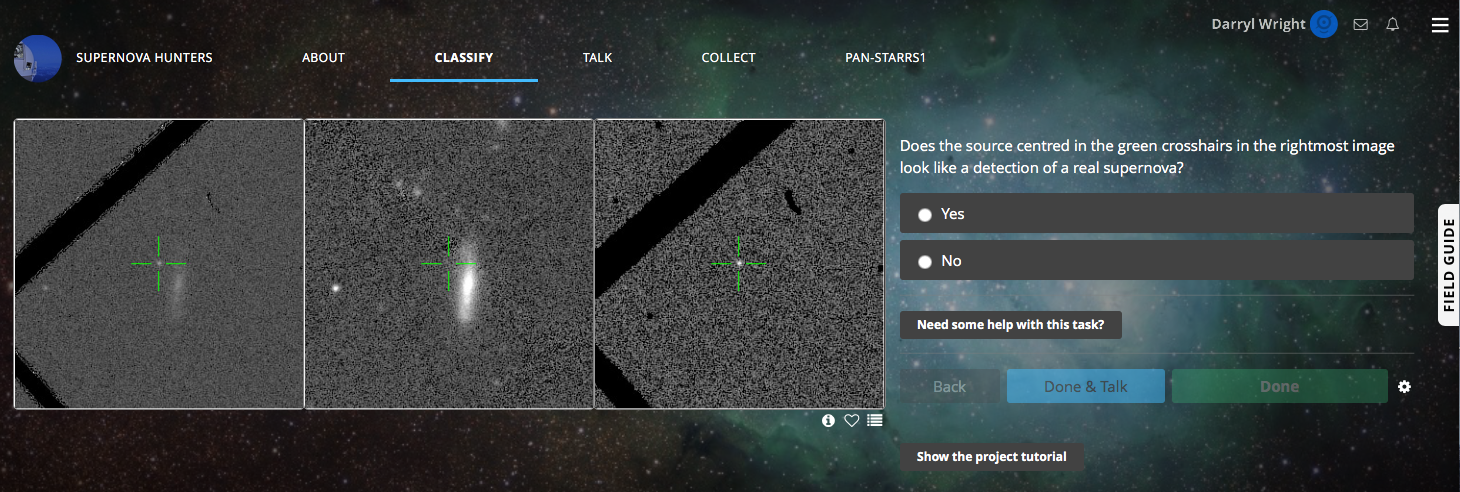
\includegraphics[width=140mm]{figs/sn_hunters.png}
   \caption{Screenshot showing the classification interface presented to citizen scientists.  The left most image is the new \textit{target} image taken recently.  In the centre is the equivalent $3\pi$ \textit{reference} image and on the right is the \textit{difference} image.  Volunteers are asked to decide whether or not they think the detection in the green crosshairs in the difference image is a
detection of a real transient.} 
   \label{fig:sn_hunters}
   \end{minipage}
\end{figure*}

Supernova Hunters was launched on the 12th July 2016 (MJD 57581).  As of the 3rd September 2016 the project has accumulated 426481 classifications from 3158 citizen scientists.  Citizen scientists are presented with the interface shown in Figure.~\ref{fig:sn_hunters} and have classified 52291 individual subjects corresponding to TTI observations (see Section~\ref{sec:ps1}) of 18838 PS1 objects. As guidance we provide a ``Field Guide'' that provides a desciption and examples of the different artefact types we expect.  Every Tuesday $\sim5200$ new subjects are uploaded to the project consisting of the previous week's detections that pass our machine cuts.  We require at least 7 citizen scientist classifications before a subject is considered classified and subsequently  retired from the project.  Since launch the project averages $\sim23000$ classifications in the first 24 hours after the data is released and $\sim8300$ classifications in the following 24 hours by which time all subjects are normally retired. High confidence (typically $P(real)>0.8$) supernova candidates are screened by experts to remove a small number of false positives before the targets are submitted to the Transient Name Server (TNS).  To date citizen scientists have discovered two hundred supernova candidates submitted to the TNS and two confirmed Supernovae including SN 2016els; a superluminous supernova Type I [XXXXX cite Gal-Yam?? XXXXX].  The classification spectra were obtained by PESSTO [XXXXX cite Smartt XXXXX].

\section{Performance}

We present the results of our machine classifier (Section~\ref{sec:cnn}) in Figure~\ref{fig:machine_dist} on PS1 data between MJD 57570 and MJD 57586. A major contaminant is the presence of asteroids; they appear in the difference image as supernovae but are identified here via cross-matching with the Minor Planet Centre ephemaris database (XXXXXX). 

These data were additionally reviewed by at least one expert members of the team (normally DW or KS) to identify genuine supernovae. Candidates were divided into `real' and `bogus' categories based on these expert classifications. 

\begin{figure}
   %\vspace{200pt}
   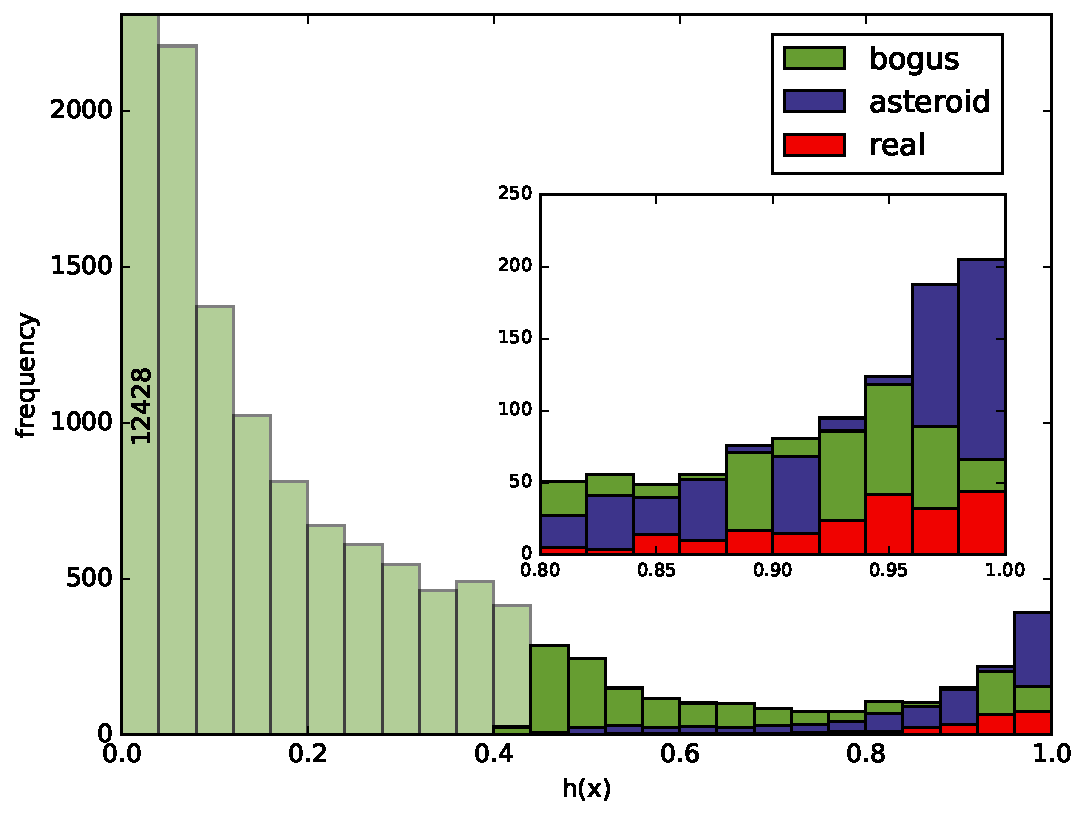
\includegraphics[width=84mm]{figs/machine_hist.pdf}
   \caption{The distribution of hypotheses, $h(x)$ from the current 3$\pi$ machine classifier 
            for detected objects between MJD 57570 and MJD 57586.  The light green shows the distribution of 
            objects with $P(real) \leq 0.436$ which are automatically rejected.  The remaining 
            objects promoted for human screening even at high values of $h(x)$ contains
            many false positives.} 
   \label{fig:machine_dist} 
\end{figure}

Candidates with high probability as assigned by the machine are more likely to be real. However, although the machine successfully rejects the majority of bogus candidates, the sample produced by the simple cut on hypothesus is far from pure; 1403 real candidates from 3384 in the sample. Higher cutoffs run the risk of rejecting an increasing number of real candidates; requiring a 1\% false positive rate will result in a missed detection rate of 60.3\%. 

An obvious solution to improve the performance of the neural network is to increase the size of the training set. This is expected to both directly improve performance but also allow for deeper, more complex networks to be built. However, it is obvious already that obtaining large, clean training sets is expensive, requiring the review of many candidates by experts. In order to reduce the burden on the science team, candidates which exceed this threshold were also classified by volunteers via the \emph{Supernova Hunters} project. The results of this analysis are shown in fig \ref{fig:human_dist}. 

\begin{figure}
   %\vspace{200pt}
   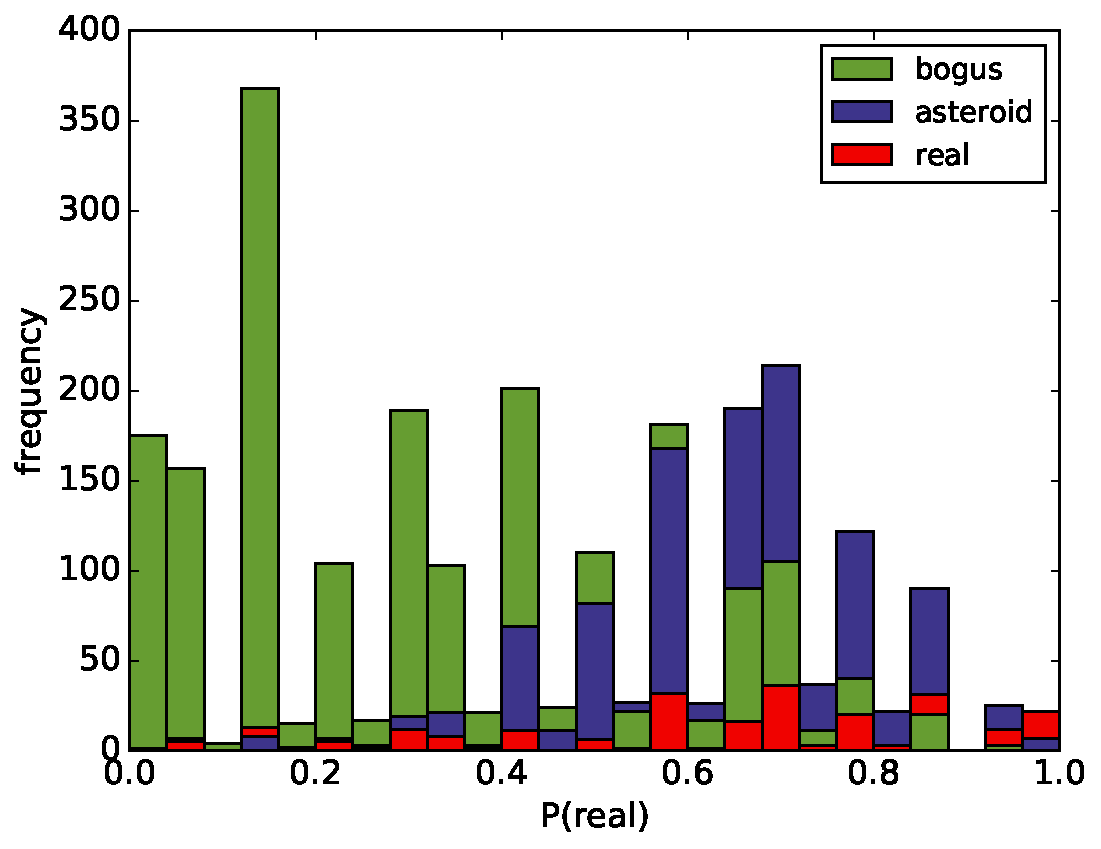
\includegraphics[width=84mm]{figs/human_hist.pdf}
   \caption{The distribution of $P(real)$ from Supernova Hunters for objects detected between 
            MJD 57570 and MJD 57586.  Compared with the machine $P(real)$ in ~\ref{fig:machine_dist}
            the objects at the extremes are pure.  There are very few real detections with 
            $P(real) < 0.04$ and few bogus detections above 0.92.} 
   \label{fig:human_dist} 
\end{figure}

Volunteer classifications were combined using the simplest possible metric; the fraction of volunteers who identified a potential transient is assumed to be an estimate of the probability of that candidate being real. Despite this simple procedure, the results show that volunteers could effectively distinguish between real and bogus classifications. However, the structure of the resulting distribution is strikingly different. Whereas for machine classification, a threshold could be chosen to give a complete but not pure sample, with volunteer classification it is easier to construct a pure sample of candidates which are highly likely to be supernovae, but this sample is far from complete. There are candidates judged `real' by experts even at low probabilities. 

Much work has been done in other projects to improve on this naive combination of volunteer votes. (XXXX Examples XXXX). However, such solutions have not yet shown to be generalisable between projects, and so require substantial effort in data analysis. They may also depend large numbers of volunteers classifying each subject. Instead of pursuing this route, therefore, we combine human and machine classifications hoping to benefit from the different capabilities of both sets of classifiers. 

\subsection{Combining human and machines} 

Figure \ref{fig:combo_train} shows the combination of human and machine classifications. It is immediately apparent from the figure that no single threshold on either machine or human classification can outperform the combination of the two. This is an important result; it is the first time that the benefits of combining classification from both machines and volunteers has been clearly demonstrated using data from a real astronomical system. 

\begin{figure}
   %\vspace{200pt}
   %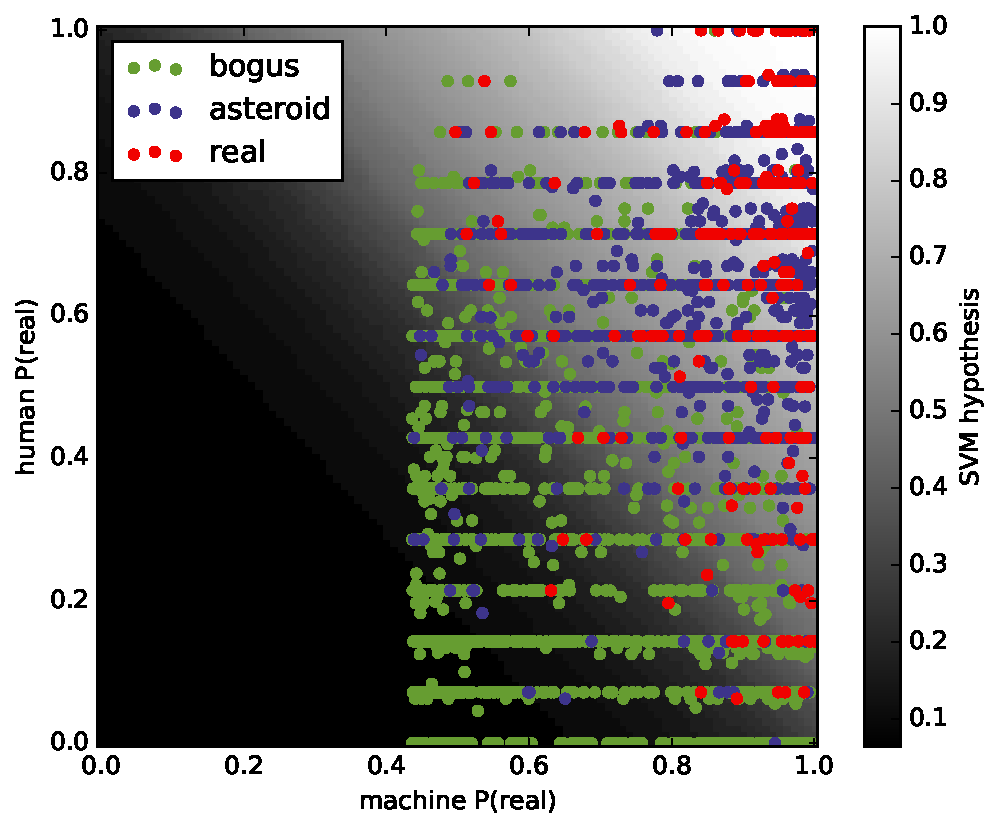
\includegraphics[width=84mm]{figs/human_v_machine_train.pdf}
   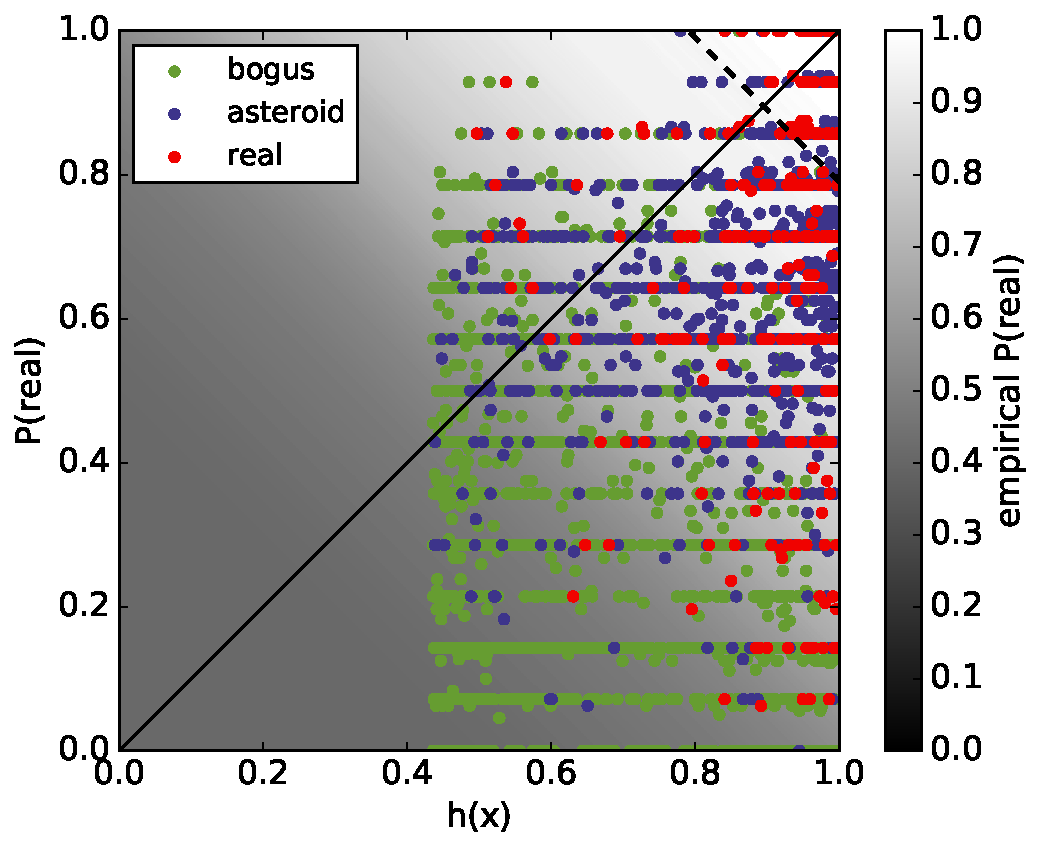
\includegraphics[width=84mm]{figs/human_v_machine_20160712-20160718.pdf}
   \caption{The $P(real)$ from Supernova Hunters against the machine $P(real)$ for detected 
            objects between MJD 57570 and MJD 57586.  $P(real)$ and $h(x)$ are combined by projecting the data onto 
             the solid black line in the euclidean sense.  For a given value of $\tau$ the background colour map
            shows the probability that an example chosen at random with combined score abouve tau will be real; an
            empirical measure of P(real) for our combination of method.  The dashed black line shows the 90\% probability contour.}
   \label{fig:combo_train} 
\end{figure}

% How should the two independent classifications be combined? We use a linear support vector machine (SVM) with inputs consisting of both classifications, trained by the expert-labelled data. 

% [XXXX put some equations XXXX]

% The SVM  maximises the distance between populations of first `real' (and `asteroid') classifications and second `bogus' classifications, using only probability estimates from humans and machines as input. It was trained on the data discussed above, and the resulting score displayed as grayscale in figure \ref{fig:combo_train}. It was then tested on data processedsed between MJD 57587 and MJD 57607, with results shown in \ref{fig:combo:test}. This test shows that the combined classification performs well, and figures \ref{fig:roc} shows a comparison of the combined results for this test dataset with machine and human classifications on their own.

How should the two independent classifications be combined?  We simply apply a decision boundary of the form $\tau = \sqrt{P(real)^2 + h(x)^2}$ over the 2D surface, where $0\leq\tau\leq1$.  This is equivalent to projecting the data onto $P(real)=h(x)$ producing a new scalar score for each detection (see Figure.~\ref{fig:combo_hist}).  Figure.~\ref{fig:combo_hist} shows the distribution of the resulting combined scores.  This distribution maintains the purity at high combined scores that we see from human classifications, but also allows a better trade-off between purity and completeness.  As an independent test we apply this same method to data between MJD 57587 and MJD 57627 in
Figure.~\ref{fig:combo_test}.  Between MJD 57609 and MJD 57615 we relaxed our cut on $h(x)$ from 0.436 to 0.3 uploading any objects passing this cut to Supernova Hunters.  This allowed the recovery of SN 2016fev at type Ia Supernova that would have been automatically rejected with $h(x)$=0.39, but which recieved a $P(real)$ of 1.0 from Supernova Hunters.  The performance of this combination method on this data set is reported in tables~\ref{tab:roc_fpr} and ~\ref{tab:roc_mdr} and the Reciever Operator Charateristic (ROC) Curve and Purity-Completeness (Precision-Recall) Curves are shown in Fig.~\ref{fig:roc}.

\begin{figure}
   %\vspace{200pt}
   %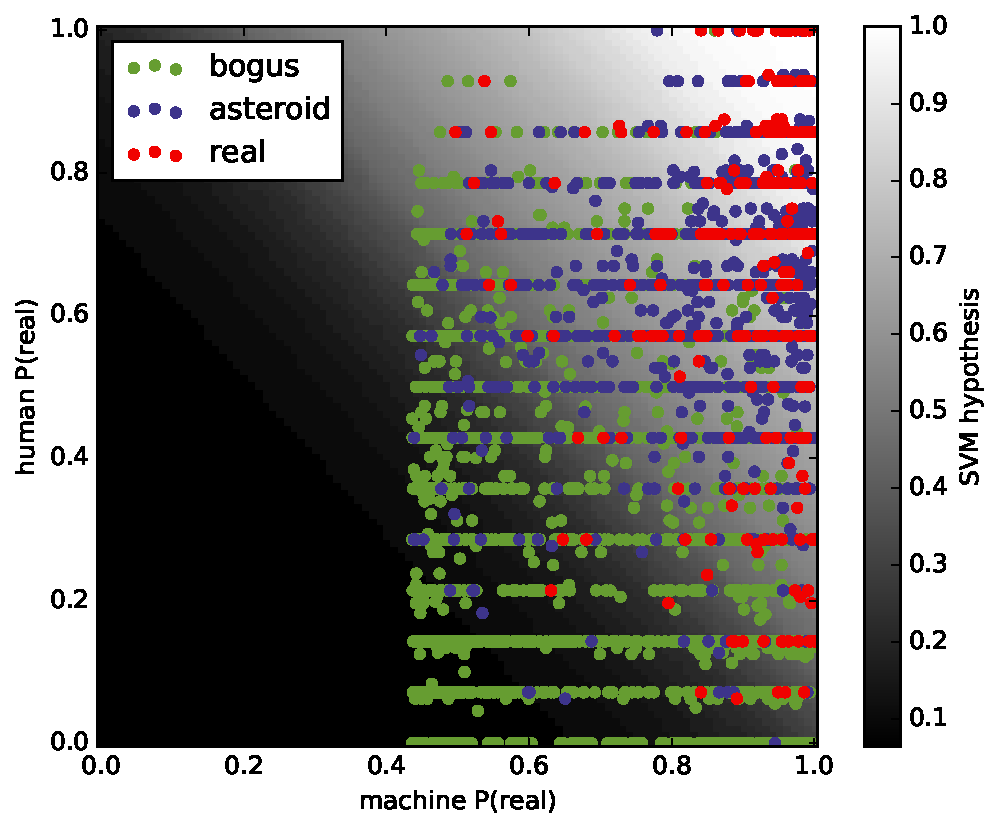
\includegraphics[width=84mm]{figs/human_v_machine_train.pdf}
   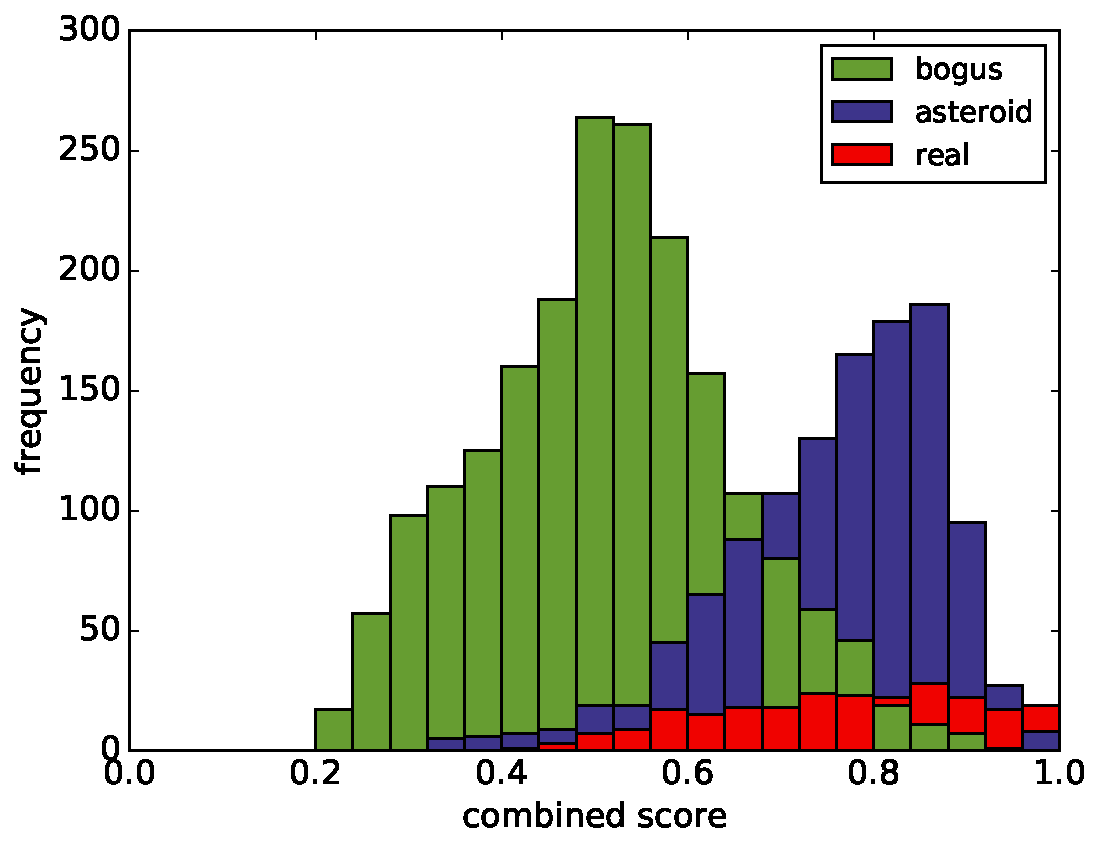
\includegraphics[width=84mm]{figs/combo_hist.pdf}
   \caption{Histogram showing the distribution of data resulting from the combination of human and machine classifications.}
   \label{fig:combo_hist} 
\end{figure}

\begin{figure}
   %\vspace{200pt}
   %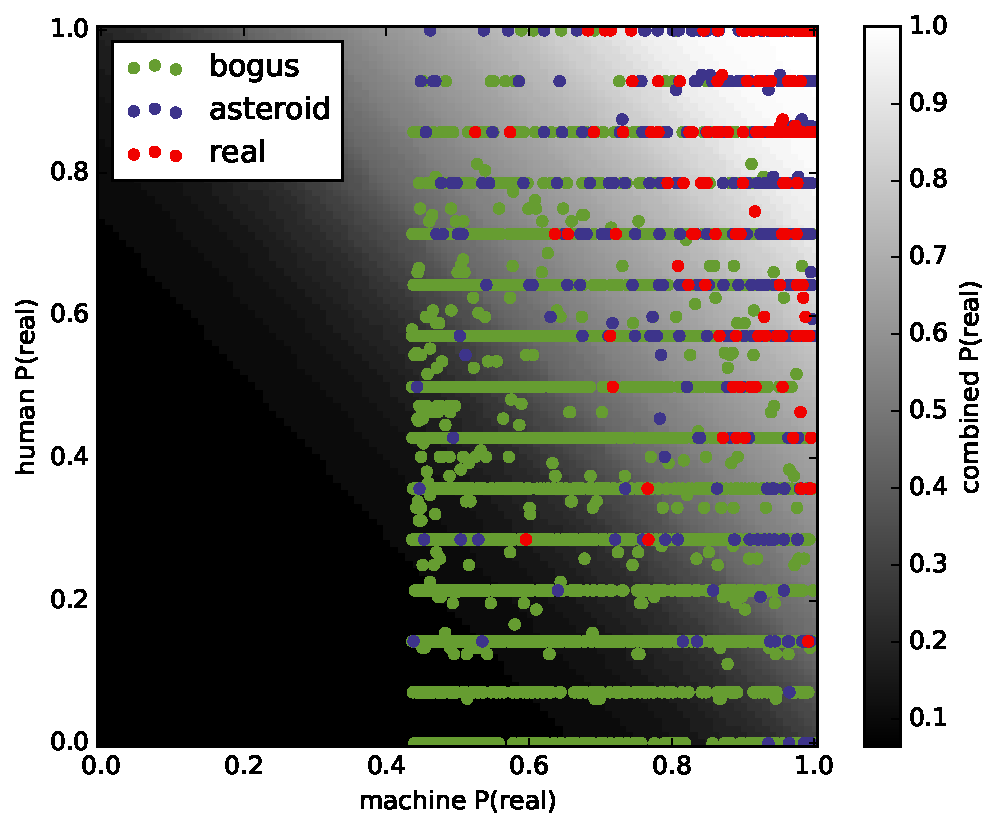
\includegraphics[width=84mons of first `real' (and `asteroid') classifications and second `bogus' classifications, using only probability estimates from humans and machines as input. It was trained on the data discussed above, and the resulting score displayed as grayscale in figure \ref{fig:combo_trainm]{figs/human_v_machine_test.pdf}
   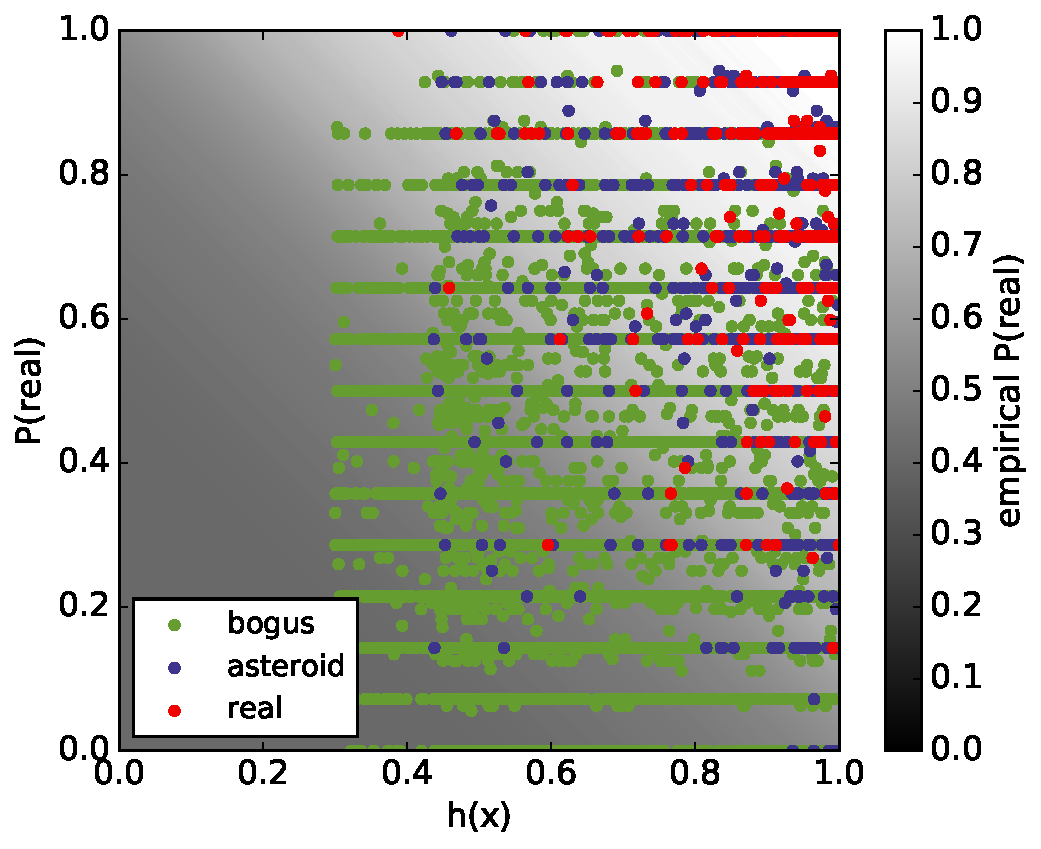
\includegraphics[width=84mm]{figs/human_v_machine_20160725-20160829.pdf}
   \caption{The same as ~\ref{fig:combo_train} but on a new sample of 10908 objects detected between
            MJD 57587 and MJD 57627.  Between we relaxed our cut on $h(x)$ to 0.3 which allowed us to recover a supernova with $h(x)$=0.39, but achieved a $P(real)$=1.0 from Supernova Hunters.  The background colour map is the same empirical $P(real)$ as Figure.~\ref{fig:combo_train} but underestimates the probability at each value of $\tau$ for this data set, perhaps suggesting an improvement in the classification ability of volunteers over time.}
   \label{fig:combo_test} 
\end{figure}

\begin{figure*}
   %\vspace{200pt}
   \begin{minipage}{140mm}
   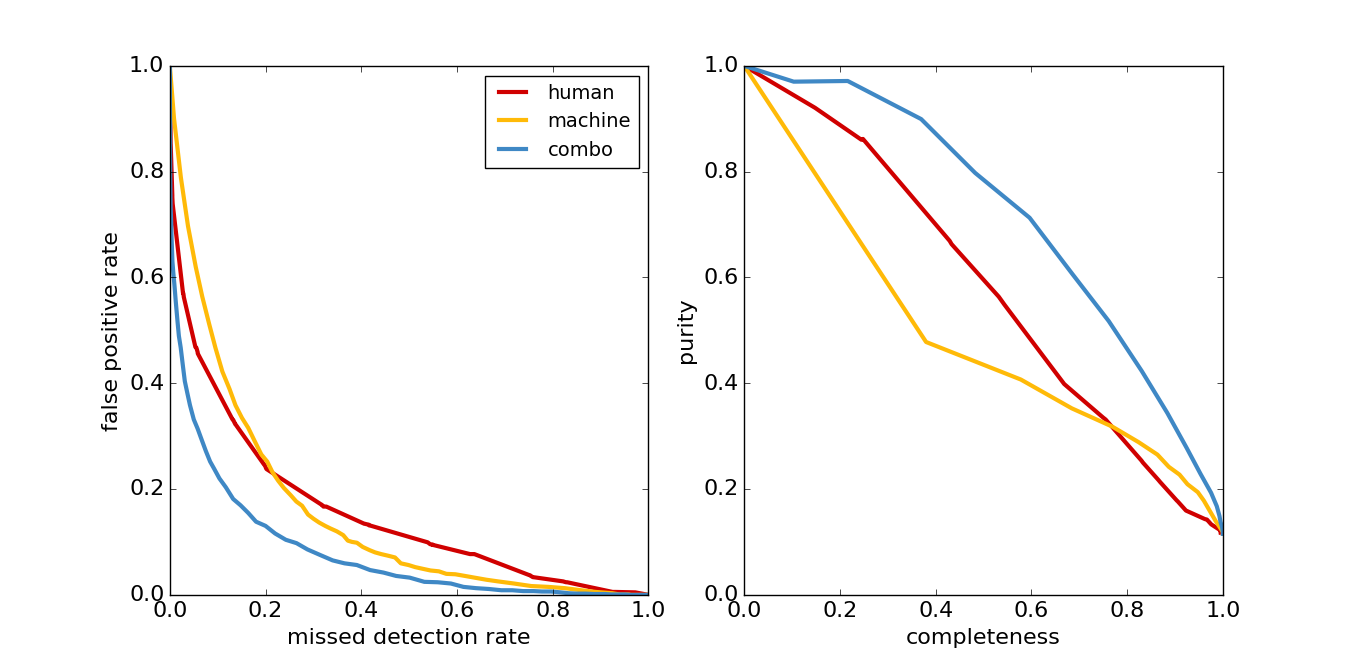
\includegraphics[trim=20mm 0mm 0mm 0mm,clip,width=150mm]{figs/roc.png}
   \caption{left: ROC curve showing performance measured on the test data in ~\ref{fig:combo_test} for human (red), machine (yellow) and
            the combination of human and machine classifications (blue).  right: The equivalent Purity-Completeness curve.  Both
            plots show that the combination always outperforms humans or the machine individually.} 
   \label{fig:roc} 
   \end{minipage}
\end{figure*}

% \begin{table}
% \begin{tabular}{|c|c|c|c|}
% FPR & Human & Machine & Combination\\
% 1\% & 65.7\% (38.3\%) & 91.1\% (49.6\%) & 55.1\% (23.8\%)\\
% 5\% & 49.4\% (12.5\%) & 64.6\% (6.8\%) & 32.2\% (4.1\%)\\
% 10\% & 38.3\% (1.1\%) & 44.9\% (1.0\%) & 22.7\% (0.2\%)\\
% \end{tabular}
% \caption{Missed detection rate recorded for a choice of false positive rates, based on expert classifications.  Figures in brackets take detections automatically rejected by the machine classifier into account and assuming that all real detections are promoted which is approximately true.}\label{tab:roc}
% \end{table}
\begin{table}
\begin{tabular}{|c|c|c|c|}
False Positive Rate & Human & Machine & Combination\\
1\% & 73.9\% & 90.1\% & 58.7\%\\
5\% & 56.3\% & 69.7\% & 35.8\%\\
10\% & 45.6\% & 46.7\% & 23.8\%\\
\end{tabular}
\caption{Missed detection rate recorded for a choice of false positive rates, based on expert classifications.}
\label{tab:roc_fpr}
\end{table}

XXXXXXXX Calculate FPR for a variety of missed detection rates XXXXXX

% \begin{table}
% \begin{tabular}{|c|c|c|c|}
% MDR & Human & Machine & Combination\\
% 1\% & 100.0\% (10.3\%)& 94.3\% (9.7\%) & 84.9\% (8.8\%) \\
% 5\% & 73.0\% (7.5\%) & 65.4\% (6.8\%) & 42.4\% (4.4\%) \\
% 10\% & 60.8\% (6.3\%) & 39.2\% (4.0\%) & 23.7\% (2.4\%) \\
% \end{tabular}
% \caption{False positive rate recorded for a choice of missed detection rates, based on expert classifications.  Figures in brackets take detections automatically rejected by the machine classifier into account.}\label{tab:roc}
% \end{table}

\begin{table}
\begin{tabular}{|c|c|c|c|}
Missed Detection Rate & Human & Machine & Combination\\
1\% & 92.5\% & 85.9\% & 69.3\% \\
5\% & 75.1\% & 52.8\% & 41.8\% \\
10\% & 53.8.8\% & 39.1\% & 26.5\% \\
\end{tabular}
\caption{False positive rate recorded for a choice of missed detection rates, based on expert classifications.
}\label{tab:roc_mdr}
\end{table}

For any choice of false positive rate, the combination of classifications produced a lower missed detection rate. Equally, for any required purity or completeness the combination provides a better trade-off. 

We have chosen to implement one of the simplest methods for combining human and machine classifications to demonstrate how they complement one another.  But it is easy to think of more complex combination methods, for example we trained a linear SVM on the data presented in Fig.~\ref{fig:combo_train} and found, unsuprisingly, that the performance measured on the data in Fig.~\ref{fig:combo_test} was typically within 1\% of the values reported in tables~\ref{tab:roc_fpr} and ~\ref{tab:roc_mdr}.  Although the gains in this example are negligible, if we wish to incorporate additional information they become important.  As an example we also have a machine score from a classifier trained on catalogue information (similar in concept to the features of \citet{Bloom12}, \citet{Brink13} and \citet{Goldstein15}) for each of the Supernova Hunters detections.  It is unlikely that the combination method presented here will work for this higher dimensional representation, but we can expect that an SVM may
gain from the added information.

\section{Conclusions}

\textbf{CJL}

\bibliographystyle{mnras} 
\bibliography{ps1_real_bogus}

\end{document}\bsp	% typesetting comment
\label{lastpage}
